% ======================================================================
%  Effective thermal conductivity from a phase field: from the sharp
%  two-domain cell problem to a diffuse formulation without first-order
%  bias.
%
%  Written to be lifted into a manuscript or thesis chapter. Scope: the
%  steady-state homogenization cell problem on a frozen phase field only.
% ======================================================================

\documentclass[11pt]{article}
\usepackage{amsmath,amssymb,amsthm,booktabs}
\usepackage{pgfplots}
\usepgfplotslibrary{fillbetween}
\pgfplotsset{compat=1.18}
\usepackage[margin=1in]{geometry}
\usepackage{microtype}
\usepackage{url}
\emergencystretch=3em

\newtheorem{lemma}{Lemma}
\newtheorem{proposition}{Proposition}

\newcommand{\Om}{\Omega}
\newcommand{\Gam}{\Gamma}
\newcommand{\bn}{\hat{\mathbf n}}
\newcommand{\bI}{\mathbf I}
\newcommand{\be}{\mathbf e}
\newcommand{\bt}{\mathbf t}
\newcommand{\bK}{\mathbf K}
\newcommand{\Keff}{\mathbf{K}_{\mathrm{eff}}}
\newcommand{\Ka}{K_{\mathrm a}}
\newcommand{\Ki}{K_{\mathrm i}}
\newcommand{\Kt}{K_{t}}
\newcommand{\Kn}{K_{n}}
\newcommand{\Hper}{H^1_{\mathrm{per}}(\Om)}
\newcommand{\avg}[1]{\big\langle #1 \big\rangle}
\newcommand{\jump}[1]{[\![\,#1\,]\!]}

\begin{document}

\begin{center}
{\large\bfseries Effective thermal conductivity from a phase field:\\[2pt]
a diffuse cell problem without first-order interface bias}
\end{center}

\begin{abstract}
\noindent We compute the effective thermal conductivity $\Keff$ of evolving snow
microstructures by solving the steady-state homogenization cell problem of
Calonne et al.\ (2011) directly on the phase field, where the ice--air
interface is a smooth tanh transition of width a few $\varepsilon$ rather than
a sharp surface. The conductivity must be interpolated across that transition,
and a matched asymptotic analysis shows that, to first order in $\varepsilon$,
the transition acts like a sharp interface with a spurious resistance to heat
crossing it and a spurious conductance along it; the standard arithmetic law
removes the second but not the first, because resistivity $1/K$ is convex in
$\varphi$. At $K_{\mathrm i}/K_{\mathrm a}\approx115$ the effect is large: for
a planar ice slab with heat flowing across it at $\varepsilon=L/50$, the
computed conductivity is $0.063$~W\,m$^{-1}$K$^{-1}$ against an exact $0.040$
for the same geometry, $59\%$ too high, and because the error scales with
$\varepsilon$ times the interface area per unit volume, which sintering
reduces, it distorts the time trend of $\Keff$ as well as its level. We remove
both terms by interpolating the conductivity arithmetically for gradients along
the interface, where the sharp solution's temperature gradient is continuous,
and harmonically for gradients across it, where the heat flux is continuous;
each choice makes its spurious term vanish exactly for the tanh profile, the
interface normal comes from $\nabla\varphi$, and the law reduces to the
pure-phase values outside the transition, so nothing is fitted and the sharp
limit is unchanged. Against closed-form sharp solutions it reproduces a planar
slab to $4\times10^{-7}$ at every width tested (the arithmetic law is
$3.8$--$59\%$ high) and a disk array to $0.006\%$ at $\varepsilon=L/800$ with
the error falling faster than second order, while the arithmetic law's error
matches our first-order prediction to within $2\%$.
\end{abstract}

% ----------------------------------------------------------------------
\section{The sharp cell problem}
\label{sec:sharp}

A periodic cell $\Om$ is split into ice $\Om_{\mathrm i}$ and air
$\Om_{\mathrm a}$, which meet on the interface $\Gam$. The conductivities
$\Ki,\Ka>0$ are constant. Let $\bn$ be the unit normal on $\Gam$ pointing into
the ice, and let $\jump{f}=f|_{\mathrm i}-f|_{\mathrm a}$ denote the jump across
$\Gam$. Following Calonne et al.\ (2011), $\Keff$ is obtained from two
cell-periodic correctors, $\bt_{\mathrm i}$ defined on the ice only and
$\bt_{\mathrm a}$ on the air only:
\begin{align}
\nabla\!\cdot\!\big(\Ki(\nabla\bt_{\mathrm i}+\bI)\big)&=\mathbf 0\ \text{in }\Om_{\mathrm i},&
\nabla\!\cdot\!\big(\Ka(\nabla\bt_{\mathrm a}+\bI)\big)&=\mathbf 0\ \text{in }\Om_{\mathrm a},
\label{eq:sharp-bulk}\\
\bt_{\mathrm i}&=\bt_{\mathrm a}\ \text{on }\Gam,&
\Ki(\nabla\bt_{\mathrm i}+\bI)\bn&=\Ka(\nabla\bt_{\mathrm a}+\bI)\bn\ \text{on }\Gam,
\label{eq:sharp-iface}
\end{align}
normalized by
$\int_{\Om_{\mathrm i}}\bt_{\mathrm i}+\int_{\Om_{\mathrm a}}\bt_{\mathrm a}=\mathbf 0$,
with
\begin{equation}
\Keff=\frac{1}{|\Om|}\left[\int_{\Om_{\mathrm i}}\Ki(\nabla\bt_{\mathrm i}+\bI)
+\int_{\Om_{\mathrm a}}\Ka(\nabla\bt_{\mathrm a}+\bI)\right].
\label{eq:sharp-keff}
\end{equation}
Column $m$ of this problem is the temperature field $T=\be_m\cdot\mathbf x+t_m$
driven by a unit mean gradient along $\be_m$. The two interface conditions are
the physics: temperature is continuous, and so is the normal heat flux. Below we
write $\mathbf q=\bK\nabla T$ for the flux, a sign convention that is standard
for the cell problem (the physical heat flux is $-\mathbf q$).

A useful consequence of \eqref{eq:sharp-iface}: on $\Gam$ the
\emph{tangential} temperature gradient $\mathbf E_t=(\bI-\bn\otimes\bn)\nabla T$
is continuous, because $T$ is, and the \emph{normal flux}
$q_n=\mathbf q\cdot\bn$ is continuous. The normal gradient and the tangential
flux jump, by the factor $\Ki/\Ka\approx115$.

% ----------------------------------------------------------------------
\section{One field on one domain}
\label{sec:glue}

Let $\chi$ be the indicator of the ice ($\chi=1$ in $\Om_{\mathrm i}$, $0$ in
$\Om_{\mathrm a}$), and define
\begin{equation}
K_\star=\Ki\chi+\Ka(1-\chi),\qquad \bt=\bt_{\mathrm i}\chi+\bt_{\mathrm a}(1-\chi).
\label{eq:glue}
\end{equation}

\paragraph{The two correctors form one $H^1$ field.} For a smooth periodic
vector field $\boldsymbol\psi$, integrating by parts on each phase gives
\[
\int_\Om\bt\,\nabla\!\cdot\boldsymbol\psi
=-\int_{\Om_{\mathrm i}}\nabla\bt_{\mathrm i}\cdot\boldsymbol\psi
 -\int_{\Om_{\mathrm a}}\nabla\bt_{\mathrm a}\cdot\boldsymbol\psi
 -\int_\Gam\jump{\bt}\,\boldsymbol\psi\cdot\bn\,d\Gam .
\]
The last term vanishes for every $\boldsymbol\psi$ if and only if
$\bt_{\mathrm i}=\bt_{\mathrm a}$ on $\Gam$. So, by the first condition in
\eqref{eq:sharp-iface}, $\bt\in\Hper$, and its gradient is the piecewise
gradient, with no part concentrated on $\Gam$. The coefficient $K_\star$ may
jump; the corrector may not.

\paragraph{One weak equation.} Multiply each bulk equation by a periodic test
function $v$, integrate by parts on its own phase, and add. The outer-boundary
terms cancel by periodicity. The interface terms combine into
$\int_\Gam v\,\jump{K(\nabla\bt+\bI)\bn}$, which vanishes by the second
condition in \eqref{eq:sharp-iface}. The two volume integrals have the same
integrand once written with $K_\star$ and the glued $\bt$, so they merge:
\begin{equation}
\int_\Om\nabla v\cdot K_\star(\nabla\bt+\bI)\,d\Om=0\quad\forall v\in\Hper,
\qquad \avg{\bt}=\mathbf 0,\qquad
\Keff=\avg{K_\star(\nabla\bt+\bI)} .
\label{eq:weak-sharp}
\end{equation}
Both steps reverse. A test function supported inside one phase returns that
phase's bulk equation, and one straddling $\Gam$ returns the flux condition. A
single $H^1$ field cannot jump, so continuity is built in. So
\eqref{eq:weak-sharp} \emph{is} the Calonne problem, written on one domain with
one unknown, and not an approximation to it.

% ----------------------------------------------------------------------
\section{The diffuse formulation}
\label{sec:diffuse}

The phase-field model does not provide $\chi$. It provides a smooth $\varphi$,
equal to $1$ in ice and $0$ in air, with the tanh profile
\begin{equation}
\varphi=\ell(s/\varepsilon)=\tfrac12\big[1+\tanh\big(s/2\varepsilon\big)\big],
\qquad \ell(u)=\frac{1}{1+e^{-u}},\qquad \ell(-u)=1-\ell(u),
\label{eq:profile}
\end{equation}
where $s$ is the signed distance to $\Gam$ (the $\varphi=\tfrac12$ level set),
positive in ice. $\ell$ is simply this profile written in the variable
$u=s/\varepsilon$.

\begin{lemma}\label{lem:any}
Let $K(\cdot)$ be any function with $K(0)=\Ka$ and $K(1)=\Ki$. Then
$K(\chi)=K_\star$ exactly.
\end{lemma}
\begin{proof}
$\chi$ only takes the values $0$ and $1$.
\end{proof}

\noindent So \eqref{eq:weak-sharp} is the equation
$\int\nabla v\cdot K(\chi)(\nabla\bt+\bI)=0$, and the diffuse formulation is the
same equation with $\chi$ replaced by $\varphi$:
\begin{equation}
\int_\Om\nabla v\cdot\bK(\varphi)\,(\nabla\bt+\bI)\,d\Om=0\quad\forall v\in\Hper,
\qquad \Keff^\varepsilon=\avg{\bK(\varphi)(\nabla\bt+\bI)} .
\label{eq:weak-diffuse}
\end{equation}
The only approximation is geometric, $\varphi$ in place of $\chi$. The lemma
also shows that the sharp problem cannot see how $\bK$ behaves for
$0<\varphi<1$. Every interpolation with the right end values gives the same
sharp limit. The choice matters only inside the transition, and there it sets
the error at finite $\varepsilon$. The standard choice is the arithmetic law
$K(\varphi)=\Ka+(\Ki-\Ka)\varphi$. The question is which interpolation makes
\eqref{eq:weak-diffuse} closest to \eqref{eq:weak-sharp}.

To answer it we allow, from the start, a coefficient that may act differently
along and across the interface:
\begin{equation}
\bK=\Kt(\varphi)\,\big(\bI-\bn\otimes\bn\big)+\Kn(\varphi)\,\bn\otimes\bn,
\qquad \bn=\frac{\nabla\varphi}{|\nabla\varphi|},
\label{eq:Kgeneral}
\end{equation}
with $\Kt,\Kn$ equal to $\Ka$ at $\varphi=0$ and $\Ki$ at $\varphi=1$. A scalar
law is the special case $\Kt=\Kn$.

\paragraph{Where this form comes from.} The outer product is a projection:
$(\bn\otimes\bn)\mathbf g=\bn(\bn\cdot\mathbf g)$ keeps the part of a vector
$\mathbf g$ along $\bn$, and $\bI-\bn\otimes\bn$ keeps the part along the
interface. So \eqref{eq:Kgeneral} says only that the normal part of the gradient
is multiplied by $\Kn$ and the tangential part by $\Kt$. It is also the
\emph{only} linear law with that property and no coupling between the two
directions. Suppose $\bK$ had a normal--tangential entry $c$. Inside the
transition the normal flux would be $\Kn\partial_sT+c\,\mathbf E_t$, and the
expansion of \S\ref{sec:inner} would give the temperature jump an extra term
$-\mathbf E_t\!\int c/\Kn\,du$, a spurious interface term beyond the two
analysed below. With $c=0$, $\bK$ is symmetric, $\bn$ is an eigenvector with
eigenvalue $\Kn$, and the directions along the interface are eigenvectors with
eigenvalue $\Kt$. A symmetric tensor with that eigenstructure is exactly
\eqref{eq:Kgeneral}. In two dimensions, with $\bn=(\cos\theta,\sin\theta)$,
\[
\bK=\begin{pmatrix}\Kt\sin^2\theta+\Kn\cos^2\theta & (\Kn-\Kt)\sin\theta\cos\theta\\
(\Kn-\Kt)\sin\theta\cos\theta & \Kt\cos^2\theta+\Kn\sin^2\theta\end{pmatrix}.
\]
Its off-diagonal entries in $x,y$ are not a coupling. They appear only because
the interface is not aligned with the axes, and in the interface's own frame
$\bK=\mathrm{diag}(\Kn,\Kt)$. For the profile \eqref{eq:profile},
$\nabla\varphi=\ell'(s/\varepsilon)\,\nabla s/\varepsilon$ is parallel to
$\nabla s$, so $\bn$ is exactly the normal to the level sets of $\varphi$, and
the phase field supplies it without any extra construction.

% ----------------------------------------------------------------------
\section{What the transition does to the solution}
\label{sec:inner}

We analyse \eqref{eq:weak-diffuse} by matched asymptotic expansions in
$\varepsilon$. Away from $\Gam$ (the \emph{outer} region), $\varphi$ is $0$ or
$1$ up to exponentially small terms, and the temperature satisfies the pure-phase
equations. Near $\Gam$ (the \emph{inner} region), use the signed distance $s$
and coordinates $\mathbf y$ along $\Gam$, and stretch $s=\varepsilon u$. The
coefficient \eqref{eq:Kgeneral} depends on $u$ only, through $\ell(u)$. In
these coordinates $\nabla\!\cdot(\bK\nabla T)=0$ reads
\begin{equation}
\varepsilon^{-2}\,\partial_u\!\big(\Kn\,\partial_uT\big)
+\varepsilon^{-1}\kappa\,\Kn\,\partial_uT
+\nabla_{\mathbf y}\!\cdot\!\big(\Kt\nabla_{\mathbf y}T\big)+O(\varepsilon)=0,
\label{eq:inner}
\end{equation}
with $\kappa$ the curvature of $\Gam$ (the sum of its principal curvatures). We assume the transition is thin
compared with the radius of curvature and with the distance to other parts of
the interface. Expand $T=T_0+\varepsilon T_1+\varepsilon^2T_2+\dots$ in the
inner region.

\paragraph{Order $\varepsilon^{-2}$: temperature is continuous.}
$\partial_u(\Kn\,\partial_uT_0)=0$, so $\Kn\partial_uT_0$ is constant in $u$.
Matching to a bounded outer field forces that constant to be zero, so $T_0$ does
not depend on $u$. At leading order the temperature, and therefore its
tangential gradient $\mathbf E_t=\nabla_{\mathbf y}T_0$, is the same at every
point across the transition.

\paragraph{Order $\varepsilon^{-1}$: normal flux is continuous.}
$\partial_u(\Kn\,\partial_uT_1)=0$ (the curvature term multiplies
$\partial_uT_0=0$), so
\begin{equation}
\Kn(\ell(u))\,\partial_uT_1=q_n(\mathbf y),\qquad
\partial_uT_1=\frac{q_n}{\Kn(\ell(u))},
\label{eq:qn}
\end{equation}
with $q_n$ the same at every point across the transition, and equal to the outer
normal flux on both sides. Inside the transition the normal gradient varies as
$1/\Kn$ while the flux stays fixed.

The equation itself thus reproduces the structure of the sharp solution: the
tangential gradient and the normal flux do not change across the transition,
exactly the quantities the sharp interface conditions keep continuous. What the
transition can alter is how much temperature drop it takes to carry $q_n$
across it, and how much flux it carries along it for a given $\mathbf E_t$.

\paragraph{First order: the effective interface conditions.} Integrating
\eqref{eq:qn} across the transition gives the total temperature change. The
outer solution, extrapolated to $\Gam$ from each side, has slopes
$q_n/\Ki$ and $q_n/\Ka$. Matching the two at the edges $u=\pm U$ of the inner
region and letting $U\to\infty$ gives the outer temperature jump
\begin{equation}
\jump{T}=\Sigma_n\,q_n,\qquad
\Sigma_n=\varepsilon\int_{-\infty}^{\infty}\!\left[\frac{1}{\Kn(\ell(u))}-\frac{1}{\Kn(H(u))}\right]du ,
\label{eq:jumpT}
\end{equation}
where $H$ is the unit step, so $\Kn(H(u))$ is the sharp conductivity $K_\star$
seen along the normal. Integrating the $O(1)$ equation of \eqref{eq:inner}
across the transition in the same way gives the outer normal-flux jump
\begin{equation}
\jump{q_n}=-\nabla_\Gam\!\cdot\!\big(\Sigma_t\,\nabla_\Gam T\big),\qquad
\Sigma_t=\varepsilon\int_{-\infty}^{\infty}\!\big[\Kt(\ell(u))-\Kt(H(u))\big]\,du .
\label{eq:jumpq}
\end{equation}
The curvature term contributes $\kappa q_n$ to both the inner and the
extrapolated outer fields, so it cancels from the jump at this order. The
integrals converge because $\ell-H$ decays exponentially.

\begin{proposition}\label{prop:equiv}
To first order in $\varepsilon$, the diffuse problem \eqref{eq:weak-diffuse}
is the sharp problem with its interface conditions \eqref{eq:sharp-iface}
replaced by \eqref{eq:jumpT}--\eqref{eq:jumpq}. $\Sigma_n$ acts as a spurious
thermal resistance across $\Gam$, and $\Sigma_t$ as a spurious conductance along
it. Consequently, the diffuse formulation reproduces the sharp one to first
order, for any microstructure, if and only if
\begin{equation}
\Sigma_t=0\quad\text{and}\quad\Sigma_n=0 .
\label{eq:conditions}
\end{equation}
\end{proposition}

\noindent If both vanish, the $O(\varepsilon)$ correction to the outer field
solves the sharp problem with zero data, so it is zero, and
$\Keff^\varepsilon-\Keff^\star=O(\varepsilon^2)$. The two numbers depend only on
the profile and on $\Kt,\Kn$. They are local properties of the transition, not
of the microstructure, so \eqref{eq:conditions} is a condition on the
interpolation alone.

% ----------------------------------------------------------------------
\section{The arithmetic law fails the normal condition}
\label{sec:excess}

\paragraph{Step 1: each excess is $\varepsilon$ times a number.} The integrals
in \eqref{eq:jumpT}--\eqref{eq:jumpq} depend only on $\Ki$, $\Ka$ and the
interpolation, not on $\varepsilon$ or the geometry. Unless one is zero, the
corresponding error is first order in $\varepsilon$.

\paragraph{Step 2: a quantity affine in $\varphi$ has zero excess.} If
$f(\varphi)=\alpha+\beta\varphi$, then
$f(\ell(u))-f(H(u))=\beta[\ell(u)-H(u)]$. By the antisymmetry in
\eqref{eq:profile}, $\ell-H$ is odd: for $u>0$,
$\ell(u)-1=-\ell(-u)$. Its integral is zero (Fig.~\ref{fig:lobes}). The
transition adds exactly as much ice on the air side of $\Gam$ as it removes on
the ice side.

\begin{figure}[ht]
\centering
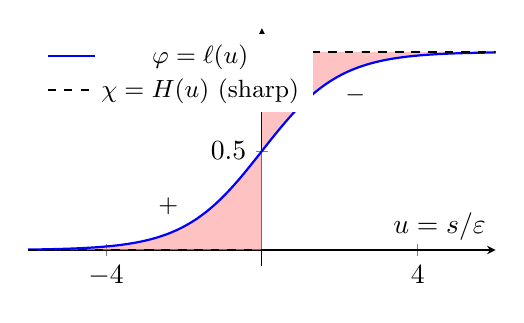
\begin{tikzpicture}
\begin{axis}[width=0.62\textwidth,height=4.6cm,xmin=-6,xmax=6,ymin=-0.08,ymax=1.12,
  axis lines=middle,xlabel={$u=s/\varepsilon$},ylabel={},xtick={-4,0,4},
  ytick={0,0.5,1},samples=200,legend style={draw=none,at={(0.02,0.98)},anchor=north west,font=\small}]
\addplot[name path=l,domain=-6:6,thick,blue]{1/(1+exp(-x))};
\addlegendentry{$\varphi=\ell(u)$}
\addplot[thick,black,dashed,domain=-6:0]{0};
\addplot[thick,black,dashed,domain=0:6]{1};
\addlegendentry{$\chi=H(u)$ (sharp)}
\path[name path=zero] (axis cs:-6,0) -- (axis cs:0,0);
\path[name path=one] (axis cs:0,1) -- (axis cs:6,1);
\addplot[red!40,opacity=0.6] fill between[of=l and zero,soft clip={domain=-6:0}];
\addplot[red!40,opacity=0.6] fill between[of=l and one,soft clip={domain=0:6}];
\node[font=\small] at (axis cs:-2.4,0.22) {$+$};
\node[font=\small] at (axis cs:2.4,0.78) {$-$};
\end{axis}
\end{tikzpicture}
\caption{The tanh profile against the sharp indicator. The two shaded regions,
$\varphi-\chi$ on either side of the interface, are mirror images with opposite
sign, so any quantity affine in $\varphi$ has zero excess.}
\label{fig:lobes}
\end{figure}

\noindent For the arithmetic law, $\Kt=\Kn=\Ka+(\Ki-\Ka)\varphi$ is affine, so
$\Sigma_t=0$. But $1/\Kn$ is not affine, and $\Sigma_n$ must be computed.

\paragraph{Step 3: computing $\Sigma_n$.} Write $a=\Ka$, $b=\Ki$, $c=b-a$, and
$K(p)=a+cp$. Substitute $p=\ell(u)$. Since $\ell'=\ell(1-\ell)$,
$du=dp/[p(1-p)]$, and $u\gtrless0$ becomes $p\gtrless\tfrac12$:
\[
\frac{\Sigma_n}{\varepsilon}
=\int_0^{1/2}\!\Big[\frac1{K}-\frac1a\Big]\frac{dp}{p(1-p)}
+\int_{1/2}^{1}\!\Big[\frac1K-\frac1b\Big]\frac{dp}{p(1-p)}
=-\frac{c}{a}\int_0^{1/2}\!\frac{dp}{K(1-p)}+\frac{c}{b}\int_{1/2}^{1}\!\frac{dp}{Kp},
\]
using $\frac1K-\frac1a=-\frac{cp}{aK}$ and $\frac1K-\frac1b=\frac{c(1-p)}{bK}$.
Partial fractions,
$\frac{1}{K(1-p)}=\frac1b\big[\frac cK+\frac1{1-p}\big]$ and
$\frac{1}{Kp}=\frac1a\big[\frac1p-\frac cK\big]$, reduce both integrals to
logarithms. With $K_m=K(\tfrac12)$, the $\ln2$ terms cancel:
\begin{equation}
\frac{\Sigma_n}{\varepsilon}=\frac{c}{ab}\Big[-\ln\frac{K_m}{a}-\ln\frac{b}{K_m}\Big]
\quad\Longrightarrow\quad
\Sigma_n^{\mathrm{arith}}=-\varepsilon\Big(\frac1\Ka-\frac1\Ki\Big)\ln\frac\Ki\Ka .
\label{eq:Sn}
\end{equation}
At $\Ki/\Ka=114.5$ the constant is $234.96$~m\,K\,W$^{-1}$. The excess is
negative because $1/K$ is convex in $\varphi$: within the transition the
arithmetic law underestimates resistivity, so the transition offers too little
resistance to heat crossing $\Gam$. It acts as a thermal short across every
interface.

\paragraph{No scalar law can satisfy both conditions.} By Step 2, $\Sigma_t=0$
calls for $K$ affine and $\Sigma_n=0$ for $1/K$ affine. Only a constant is both.
The harmonic law $1/K=\varphi/\Ki+(1-\varphi)/\Ka$ fixes the normal condition
and breaks the tangential one:
$\Sigma_t^{\mathrm{harm}}=-\varepsilon(\Ki-\Ka)\ln(\Ki/\Ka)$, by the same
calculation with $K$ and $1/K$ exchanged. Both values were checked against direct
quadrature.

% ----------------------------------------------------------------------
\section{The tensor law}
\label{sec:tensor}

Proposition~\ref{prop:equiv} asks for two separate things. Along the interface,
$\mathbf E_t$ is fixed and the transition carries flux $\Kt\mathbf E_t$, so its
total conductance must match the sharp one: $\Kt$ must average correctly. Across
the interface, $q_n$ is fixed and the temperature drop is $q_n\int ds/\Kn$, so
its total resistance must match the sharp one: $1/\Kn$ must average correctly.
The general coefficient \eqref{eq:Kgeneral} lets us meet each requirement with
its own function. By Step 2, the simplest choices are $\Kt$ affine and $1/\Kn$
affine:
\begin{equation}
\boxed{\;
\bK(\varphi,\nabla\varphi)=\underbrace{\big[\Ka+(\Ki-\Ka)\varphi\big]}_{\Kt}\big(\bI-\bn\otimes\bn\big)
+\underbrace{\Big[\frac{\varphi}{\Ki}+\frac{1-\varphi}{\Ka}\Big]^{-1}}_{\Kn}\bn\otimes\bn,
\qquad \bn=\frac{\nabla\varphi}{|\nabla\varphi|}.\;}
\label{eq:tensor}
\end{equation}
Then $\Sigma_t=\Sigma_n=0$ identically, the effective interface conditions
\eqref{eq:jumpT}--\eqref{eq:jumpq} reduce to the sharp ones, and
$\Keff^\varepsilon-\Keff^\star=O(\varepsilon^2)$.

\paragraph{Why this is the right fix.}
\begin{enumerate}
\item \emph{It targets the actual error.} Proposition~\ref{prop:equiv} shows the
first-order error consists of exactly two terms, and \eqref{eq:tensor} sets each
of them to zero. It is not a fit to any geometry.
\item \emph{It needs direction dependence, and only that.} No scalar law can
satisfy both conditions (\S\ref{sec:excess}). The tensor form is the minimal
extension: it keeps the standard arithmetic law along the interface and changes
only the response to normal gradients.
\item \emph{It is robust to the profile.} The zero excesses rely only on the
antisymmetry $\ell(-u)=1-\ell(u)$, not on the particular tanh shape. More
generally, $\Sigma_t=0$ holds for any $\Kt$ with
$\Kt(p)+\Kt(1-p)=\Ka+\Ki$, and $\Sigma_n=0$ for any $\Kn$ with
$1/\Kn(p)+1/\Kn(1-p)=1/\Ka+1/\Ki$. The affine choices are the simplest members
of these families.
\item \emph{It leaves the sharp problem untouched.} Both branches take the
pure-phase values at $\varphi\in\{0,1\}$, so $\bK=K_\star\bI$ outside the
transition and Lemma~\ref{lem:any} still holds. The sharp limit is unchanged.
\item \emph{It is well posed with the same bounds.} $\bK$ is symmetric with
eigenvalues $\Kt$ (along) and $\Kn$ (across), both in $[\Ka,\Ki]$. The cell
problem stays uniformly elliptic, $\Keff^\varepsilon$ is symmetric positive
definite, and the discrete operator stays symmetric positive definite.
\item \emph{It has no free parameter} and uses only $\varphi$ and $\nabla\varphi$,
which the phase field already provides. Where $\nabla\varphi=0$, $\bn$ is
undefined, but that happens only in the pure phases, where $\Kt=\Kn$ and $\bK$
is isotropic whatever $\bn$ is.
\end{enumerate}

% ----------------------------------------------------------------------
\section{Size of the arithmetic-law bias}
\label{sec:size}

Let $T^\star$ be the sharp solution for a unit mean gradient $\be$, and
$\mathbf E_t$, $q_n$ its tangential gradient and normal flux on $\Gam$. The
first-order correction $\tau=T^\varepsilon-T^\star$ solves the sharp bulk
equations with jumps \eqref{eq:jumpT}--\eqref{eq:jumpq}. Two applications of
the divergence theorem, one against $T^\star$ and one against its corrector,
plus the flux $\Sigma_t\mathbf E_t$ carried along $\Gam$, give
\begin{equation}
\be\cdot\Keff^{\varepsilon}\be-\be\cdot\Keff^{\star}\be
=\frac{1}{|\Om|}\int_\Gam\Big(\Sigma_t\,|\mathbf E_t|^2-\Sigma_n\,q_n^2\Big)\,d\Gam
+O(\varepsilon^2).
\label{eq:bias}
\end{equation}
For the arithmetic law only the second term survives, and since $\Sigma_n<0$
the bias is positive. The cell conducts too well wherever heat crosses an
interface, in proportion to $\varepsilon$, to the interfacial area, and to the
square of the normal flux.

\paragraph{Planar slab: the exact diffuse solution.} Take an ice slab with
two flat faces per period $L$, and $\varphi$ a function of $y$ only. The
cell problem is then one-dimensional and solvable exactly for any $\varepsilon$.
Along the faces, $t=0$ and $k_\parallel=\avg{\Kt}$. Across them,
$\Kn(t'+1)$ is constant and $\avg{t'}=0$, so $k_\perp=\avg{1/\Kn}^{-1}$. For
the arithmetic law, Step 2 gives $\avg{\Kt}$ equal to its sharp value at every
$\varepsilon$, while
\begin{equation}
\avg{1/\Kn}=\frac{\bar\varphi}{\Ki}+\frac{1-\bar\varphi}{\Ka}+\frac{2\,\Sigma_n}{L}
\label{eq:slab}
\end{equation}
up to exponentially small overlap between the two faces' tails. This is exact
in resistivity, and \eqref{eq:bias} is its linearization in $\varepsilon$. For the tensor law, $1/\Kn$ is affine and
$k_\perp$ is exact at every $\varepsilon$. At $\bar\varphi=\tfrac12$:

\begin{center}
\begin{tabular}{@{}lrrr@{}}
\toprule
$\varepsilon$ & arithmetic $k_\perp$ & exact $k_\perp$ & bias\\
\midrule
$L/50$  & $0.0632$ & $0.03965$ & $+59.4\%$\\
$L/128$ & $0.0464$ & $0.03965$ & $+17.0\%$\\
$L/512$ & $0.0412$ & $0.03965$ & $+3.8\%$\\
\bottomrule
\end{tabular}
\end{center}

\noindent The $59\%$ means that the arithmetic diffuse cell reports a
conductivity across the slab of $0.063$~W\,m$^{-1}$K$^{-1}$ for a geometry whose
true value is $0.040$. The microstructure is the same; only the numerical width
of its interfaces differs.

% ----------------------------------------------------------------------
\section{Verification}
\label{sec:verify}

Two cells with closed-form sharp solutions, run over an $\varepsilon$ ladder at
fixed $\varepsilon/h=5.12$, so the interface error is not confounded with mesh
convergence.

\paragraph{Planar slab} ($\bar\varphi=\tfrac12$). The normal is a fixed axis,
so this case tests the normal branch of \eqref{eq:tensor} in isolation.

\begin{center}
\begin{tabular}{@{}lrr@{}}
\toprule
$\varepsilon$ & arithmetic (exact, \eqref{eq:slab}) & tensor (measured)\\
\midrule
$L/50$  & $+59.4\%$ & $<4\times10^{-7}$\\
$L/64$  & $+41.1\%$ & $<4\times10^{-7}$\\
$L/128$ & $+17.0\%$ & $<4\times10^{-7}$\\
$L/256$ & $+7.9\%$  & $<4\times10^{-7}$\\
$L/512$ & $+3.8\%$  & $<4\times10^{-7}$\\
\bottomrule
\end{tabular}
\end{center}

\noindent The tensor law reproduces the exact $k_\perp$ to solver precision at
every rung, and $k_\parallel$ to $8\times10^{-7}$. The fitted slope of $1/k_\perp$
against $\varepsilon$ is $10^{-6}$ of the arithmetic law's.

\paragraph{Disk array} (square array, $f=\pi R^2/L^2=0.196$). Here the normal
takes every direction, so the full tensor, including its off-diagonal terms, is
exercised. The sharp value is Rayleigh's, $k=0.0295684$~W\,m$^{-1}$K$^{-1}$
(Rayleigh 1892; Perrins et al.\ 1979). Putting the sharp dipole field into
\eqref{eq:bias} predicts the arithmetic law's first-order slope with no fitted
constant,
\begin{equation}
\frac{dk}{d\varepsilon}=\frac{|\Sigma_n|}{\varepsilon}\,\frac{\pi R}{L^2}
\left[\frac{\Ka(1+\beta)}{1-\beta f}\right]^2,\qquad
\beta=\frac{\Ki-\Ka}{\Ki+\Ka}.
\label{eq:diskslope}
\end{equation}

\begin{center}
\begin{tabular}{@{}lrrrr@{}}
\toprule
$\varepsilon$ & arith.\ (pred.) & arith.\ (meas.) & tensor (meas.) & tensor order\\
\midrule
$L/100$ & $+15.07\%$ & $+18.19\%$ & $+1.212\%$ & \\
$L/200$ & $+7.53\%$  & $+8.26\%$  & $+0.204\%$ & $2.57$\\
$L/400$ & $+3.77\%$  & $+3.95\%$  & $+0.034\%$ & $2.59$\\
$L/800$ & $+1.88\%$  & $+1.93\%$  & $+0.006\%$ & $2.50$\\
\bottomrule
\end{tabular}
\end{center}

\noindent The arithmetic law's fitted first-order slope is within $1.9\%$ of
\eqref{eq:diskslope}, which confirms \eqref{eq:bias} on a curved interface. The
tensor law's error is at most $0.067\times$ the arithmetic error and falls at an
observed order of about $2.5$, so no first-order term remains. The measured ice
fraction equals the exact diffuse-disk value $f(1+\pi^2\varepsilon^2/3R^2)$ to
$3\times10^{-10}$, so the errors come from the conductivity law, not from the
initial condition. Drivers:
\verb|enceladus_DSM/studies/keff_sharp_limit/{verification,disk}/|.

% ----------------------------------------------------------------------
\section{Implementation}
\label{sec:code}

The cell problem \eqref{eq:weak-diffuse} is solved with isogeometric Galerkin
discretisation (PetIGA) in \verb|enceladus_dsm|, in-line with \verb|-keff 1|
or on saved snapshots with \verb|-keff_replay|. The law is selected with
\verb|-keff_interp tensor| (the default) or \verb|arith|. At each quadrature
point, \verb|KeffPointCond| builds
$\bK=\Kt\bI+(\Kn-\Kt)\,\nabla\varphi\otimes\nabla\varphi/|\nabla\varphi|^2$
from the projected $\varphi$ and $\nabla\varphi$. The stiffness
$\int\nabla N_a\cdot\bK\nabla N_b$ is assembled once and shared by all
directions. The load is $-\int\nabla N_a\cdot\bK\be_m$, and $\Keff$ is the
quadrature average of $\bK(\nabla t_m+\be_m)$.

% ----------------------------------------------------------------------
\section{Scope and limitations}
\label{sec:scope}

\begin{itemize}
\item \emph{Steady state only.} Everything here concerns the homogenization
cell problem on a frozen $\varphi$. It says nothing about, and is not an
argument for changing, the transient equations of the phase-field model that
produced $\varphi$.
\item \emph{Residual $O(\varepsilon^2)$.} This includes curvature terms and a
geometric one: a diffuse disk holds $\pi^3\varepsilon^2/3$ more area of ice than
the sharp disk. The observed rate on the disk is about $2.5$. We have not
derived the second-order coefficient, so the rate is an observation.
\item \emph{Thin necks.} The inner analysis assumes the transition is thin
compared with the curvature radius and with the distance to other parts of the
interface. Where two interfaces come within a few $\varepsilon$ of each other,
as in young sinter necks, the transitions overlap and no interpolation law is
justified by it. This limits how well the phase field resolves the geometry, and
it applies to the phase-field geometry as much as to $\Keff$.
\item \emph{Profile.} The argument uses the antisymmetry of the profile about
$\varphi=\tfrac12$. A profile distorted by the phase-field evolution changes the
excesses only in proportion to its departure from antisymmetry.
\item \emph{Geometry error is untouched.} The law removes the error of
homogenizing a given $\varphi$. It does not correct errors in $\varphi$ itself.
\end{itemize}

% ----------------------------------------------------------------------
\section{Related work}

\begin{itemize}
\item The expansion of \S\ref{sec:inner} is the standard thin-interface
analysis of phase-field models (Karma \& Rappel 1998). The first-order interface
corrections that arise with unequal conductivities in the two phases are
analysed by Almgren (1999) and McFadden, Wheeler \& Anderson (2000).
\item Elliptic problems posed on a smoothed indicator are the setting of the
diffuse-domain method. Li et al.\ (2009) introduce it, and Lervåg \& Lowengrub
(2015) use matched asymptotics to show which formulations are first- or
second-order accurate in $\varepsilon$.
\item In phase-field elasticity, Durga, Wollants \& Moelans (2013) show that
interpolating the stiffness creates interfacial excess contributions. Schneider
et al.\ (2015) remove them by interpolating so that the mechanical jump
conditions (continuous normal traction and tangential strain) hold inside the
diffuse interface. That is the elastic counterpart of keeping $q_n$ and
$\mathbf E_t$ continuous here.
\end{itemize}

% ----------------------------------------------------------------------
\section{Suggested Methods text}

\begin{quote}\small
The effective conductivity tensor is obtained by periodic homogenization
(Calonne et al., 2011). The two-domain cell problem is written as a single weak
equation with the piecewise conductivity $K_\star=K(\chi)$ of the ice indicator
$\chi$, and solved on the phase field by replacing $\chi$ with $\varphi$. Inside
the diffuse interface the conductivity must be interpolated. A matched
asymptotic expansion shows that, to first order in the interface width
$\varepsilon$, the diffuse interface acts as a sharp one with a spurious thermal
resistance $\Sigma_n$ across it and a spurious conductance $\Sigma_t$ along it,
both computable in closed form for the tanh profile. The arithmetic
interpolation gives $\Sigma_t=0$ but
$\Sigma_n=-\varepsilon(K_a^{-1}-K_i^{-1})\ln(K_i/K_a)$, which overestimates
conduction across interfaces by up to tens of percent at $K_i/K_a\approx115$. We
therefore use arithmetic interpolation for gradients along the interface and
harmonic interpolation for gradients across it,
$\mathbf K=K_{\mathrm{ar}}(\varphi)(\mathbf I-\hat{\mathbf n}\otimes\hat{\mathbf n})
+K_{\mathrm h}(\varphi)\,\hat{\mathbf n}\otimes\hat{\mathbf n}$ with
$\hat{\mathbf n}=\nabla\varphi/|\nabla\varphi|$. This makes both terms vanish, so
the error is $O(\varepsilon^2)$. The law reduces to the pure-phase
conductivities outside the interface and has no adjustable parameters. We
verified it against closed-form sharp solutions for a planar slab and a square
array of disks (Rayleigh, 1892; Perrins et al., 1979).
\end{quote}

\section*{References}
{\small
\noindent Almgren, R.\ F.\ (1999). Second-order phase field asymptotics for
unequal conductivities. \emph{SIAM J.\ Appl.\ Math.} 59, 2086--2107.
doi:10.1137/S0036139997330027.\\
Calonne, N., Flin, F., Morin, S., Lesaffre, B., Rolland du Roscoat, S., \&
Geindreau, C.\ (2011). Numerical and experimental investigations of the
effective thermal conductivity of snow. \emph{Geophys.\ Res.\ Lett.} 38,
L23501. doi:10.1029/2011GL049234.\\
Durga, A., Wollants, P., \& Moelans, N.\ (2013). Evaluation of interfacial
excess contributions in different phase-field models for elastically
inhomogeneous systems. \emph{Modelling Simul.\ Mater.\ Sci.\ Eng.} 21, 055018.
doi:10.1088/0965-0393/21/5/055018.\\
Karma, A., \& Rappel, W.-J.\ (1998). Quantitative phase-field modeling of
dendritic growth in two and three dimensions. \emph{Phys.\ Rev.\ E} 57,
4323--4349. doi:10.1103/PhysRevE.57.4323.\\
Lervåg, K.\ Y., \& Lowengrub, J.\ (2015). Analysis of the diffuse-domain
method for solving PDEs in complex geometries. \emph{Commun.\ Math.\ Sci.} 13,
1473--1500. doi:10.4310/CMS.2015.v13.n6.a6.\\
Li, X., Lowengrub, J., Rätz, A., \& Voigt, A.\ (2009). Solving PDEs in complex
geometries: a diffuse domain approach. \emph{Commun.\ Math.\ Sci.} 7, 81--107.
doi:10.4310/CMS.2009.v7.n1.a4.\\
McFadden, G.\ B., Wheeler, A.\ A., \& Anderson, D.\ M.\ (2000). Thin
interface asymptotics for an energy/entropy approach to phase-field models with
unequal conductivities. \emph{Physica D} 144, 154--168.
doi:10.1016/S0167-2789(00)00064-6.\\
Perrins, W.\ T., McKenzie, D.\ R., \& McPhedran, R.\ C.\ (1979). Transport
properties of regular arrays of cylinders. \emph{Proc.\ R.\ Soc.\ Lond.\ A}
369, 207--225. doi:10.1098/rspa.1979.0160.\\
Rayleigh, Lord (1892). On the influence of obstacles arranged in rectangular
order upon the properties of a medium. \emph{Phil.\ Mag.} 34, 481--502.
doi:10.1080/14786449208620364.\\
Schneider, D., Tschukin, O., Choudhury, A., Selzer, M., Böhlke, T., \&
Nestler, B.\ (2015). Phase-field elasticity model based on mechanical jump
conditions. \emph{Comput.\ Mech.} 55, 887--901. doi:10.1007/s00466-015-1141-6.
}

\end{document}
